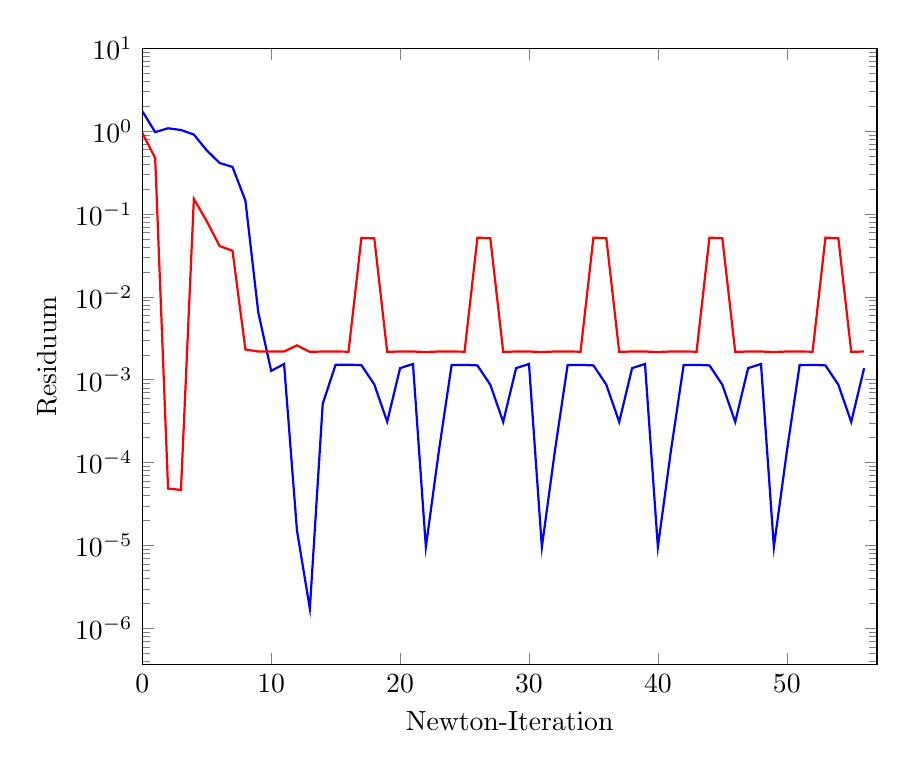
\begin{tikzpicture}[every plot/.append style={thick}] 
\begin{axis}[ 
label style={font=\normalsize}, 
xlabel={Newton-Iteration}, 
ylabel={Residuum}, 
xmin=0, xmax=57, 
ymode=log, 
ymin=0, ymax=10, 
width=0.9\textwidth, 
grid style=dashed, 
] 
\addplot[ 
color=blue, 
] 
coordinates { 
(0, 1.74e+00)(1, 9.72e-01)(2, 1.08e+00)(3, 1.03e+00)(4, 9.08e-01)(5, 5.85e-01)(6, 4.12e-01)(7, 3.69e-01)(8, 1.45e-01)(9, 6.48e-03)(10, 1.28e-03)(11, 1.55e-03)(12, 1.52e-05)(13, 1.73e-06)(14, 5.14e-04)(15, 1.52e-03)(16, 1.52e-03)(17, 1.50e-03)(18, 8.78e-04)(19, 3.12e-04)(20, 1.38e-03)(21, 1.55e-03)(22, 9.60e-06)(23, 1.35e-04)(24, 1.51e-03)(25, 1.51e-03)(26, 1.49e-03)(27, 8.71e-04)(28, 3.10e-04)(29, 1.38e-03)(30, 1.55e-03)(31, 9.60e-06)(32, 1.35e-04)(33, 1.51e-03)(34, 1.51e-03)(35, 1.49e-03)(36, 8.71e-04)(37, 3.10e-04)(38, 1.38e-03)(39, 1.55e-03)(40, 9.60e-06)(41, 1.35e-04)(42, 1.51e-03)(43, 1.51e-03)(44, 1.49e-03)(45, 8.71e-04)(46, 3.10e-04)(47, 1.38e-03)(48, 1.55e-03)(49, 9.60e-06)(50, 1.35e-04)(51, 1.51e-03)(52, 1.51e-03)(53, 1.49e-03)(54, 8.71e-04)(55, 3.10e-04)(56, 1.38e-03)}; 
\addplot[ 
color=red, 
] 
coordinates { 
(0, 9.49e-01)(1, 4.74e-01)(2, 4.87e-05)(3, 4.69e-05)(4, 1.52e-01)(5, 8.20e-02)(6, 4.10e-02)(7, 3.60e-02)(8, 2.32e-03)(9, 2.19e-03)(10, 2.19e-03)(11, 2.19e-03)(12, 2.60e-03)(13, 2.17e-03)(14, 2.19e-03)(15, 2.19e-03)(16, 2.18e-03)(17, 5.15e-02)(18, 5.08e-02)(19, 2.17e-03)(20, 2.19e-03)(21, 2.19e-03)(22, 2.16e-03)(23, 2.19e-03)(24, 2.19e-03)(25, 2.18e-03)(26, 5.18e-02)(27, 5.10e-02)(28, 2.17e-03)(29, 2.19e-03)(30, 2.19e-03)(31, 2.16e-03)(32, 2.19e-03)(33, 2.19e-03)(34, 2.18e-03)(35, 5.18e-02)(36, 5.10e-02)(37, 2.17e-03)(38, 2.19e-03)(39, 2.19e-03)(40, 2.16e-03)(41, 2.19e-03)(42, 2.19e-03)(43, 2.18e-03)(44, 5.18e-02)(45, 5.10e-02)(46, 2.17e-03)(47, 2.19e-03)(48, 2.19e-03)(49, 2.16e-03)(50, 2.19e-03)(51, 2.19e-03)(52, 2.18e-03)(53, 5.18e-02)(54, 5.10e-02)(55, 2.17e-03)(56, 2.19e-03)}; 
\end{axis} 
\end{tikzpicture} 
